\documentclass[tikz,border=12pt]{standalone}
\usepackage[utf8]{inputenc}
\usepackage[T1]{fontenc}
\usepackage{amsmath,amssymb}
\usepackage{tikz}
\usetikzlibrary{arrows.meta,positioning,fit,calc,backgrounds,shapes.geometric}

% V6 pastel-first palette
\definecolor{CoreNavy}{RGB}{72,92,120}
\definecolor{MutedBlue}{RGB}{104,132,164}
\definecolor{MutedRust}{RGB}{174,112,96}
\definecolor{MutedTeal}{RGB}{92,146,142}
\definecolor{PaleBlue}{RGB}{235,241,247}
\definecolor{PaleTeal}{RGB}{232,244,242}
\definecolor{PalePeach}{RGB}{248,238,231}
\definecolor{PaleRose}{RGB}{247,235,235}
\definecolor{SoftGray}{RGB}{244,245,246}
\definecolor{MidGray}{RGB}{153,160,168}
\definecolor{Ink}{RGB}{40,45,52}

\tikzset{
  >={Stealth[length=2.0mm,width=1.4mm]},
  every path/.style={line cap=round,line join=round},
  module/.style={
    draw=CoreNavy,
    fill=white,
    line width=0.85pt,
    rounded corners=2.2mm,
    align=center,
    inner xsep=2.5mm,
    inner ysep=2.2mm,
    minimum height=14mm,
    text width=46mm,
    font=\sffamily\footnotesize,
    text=Ink
  },
  primary/.style={module,fill=PaleBlue},
  context/.style={module,draw=MutedTeal,fill=PaleTeal},
  caution/.style={module,draw=MutedRust,fill=PalePeach},
  neutral/.style={module,draw=MidGray,fill=SoftGray},
  group/.style={draw=MidGray,dashed,line width=0.8pt,rounded corners=3mm,inner sep=6.0mm},
  flow/.style={->,draw=CoreNavy,line width=0.95pt},
  contextual-flow/.style={->,draw=MutedTeal,line width=1.0pt,dashed},
  caution-flow/.style={->,draw=MutedRust,line width=1.0pt},
  label/.style={font=\sffamily\footnotesize,text=Ink,align=center,inner sep=0pt}
}

\begin{document}
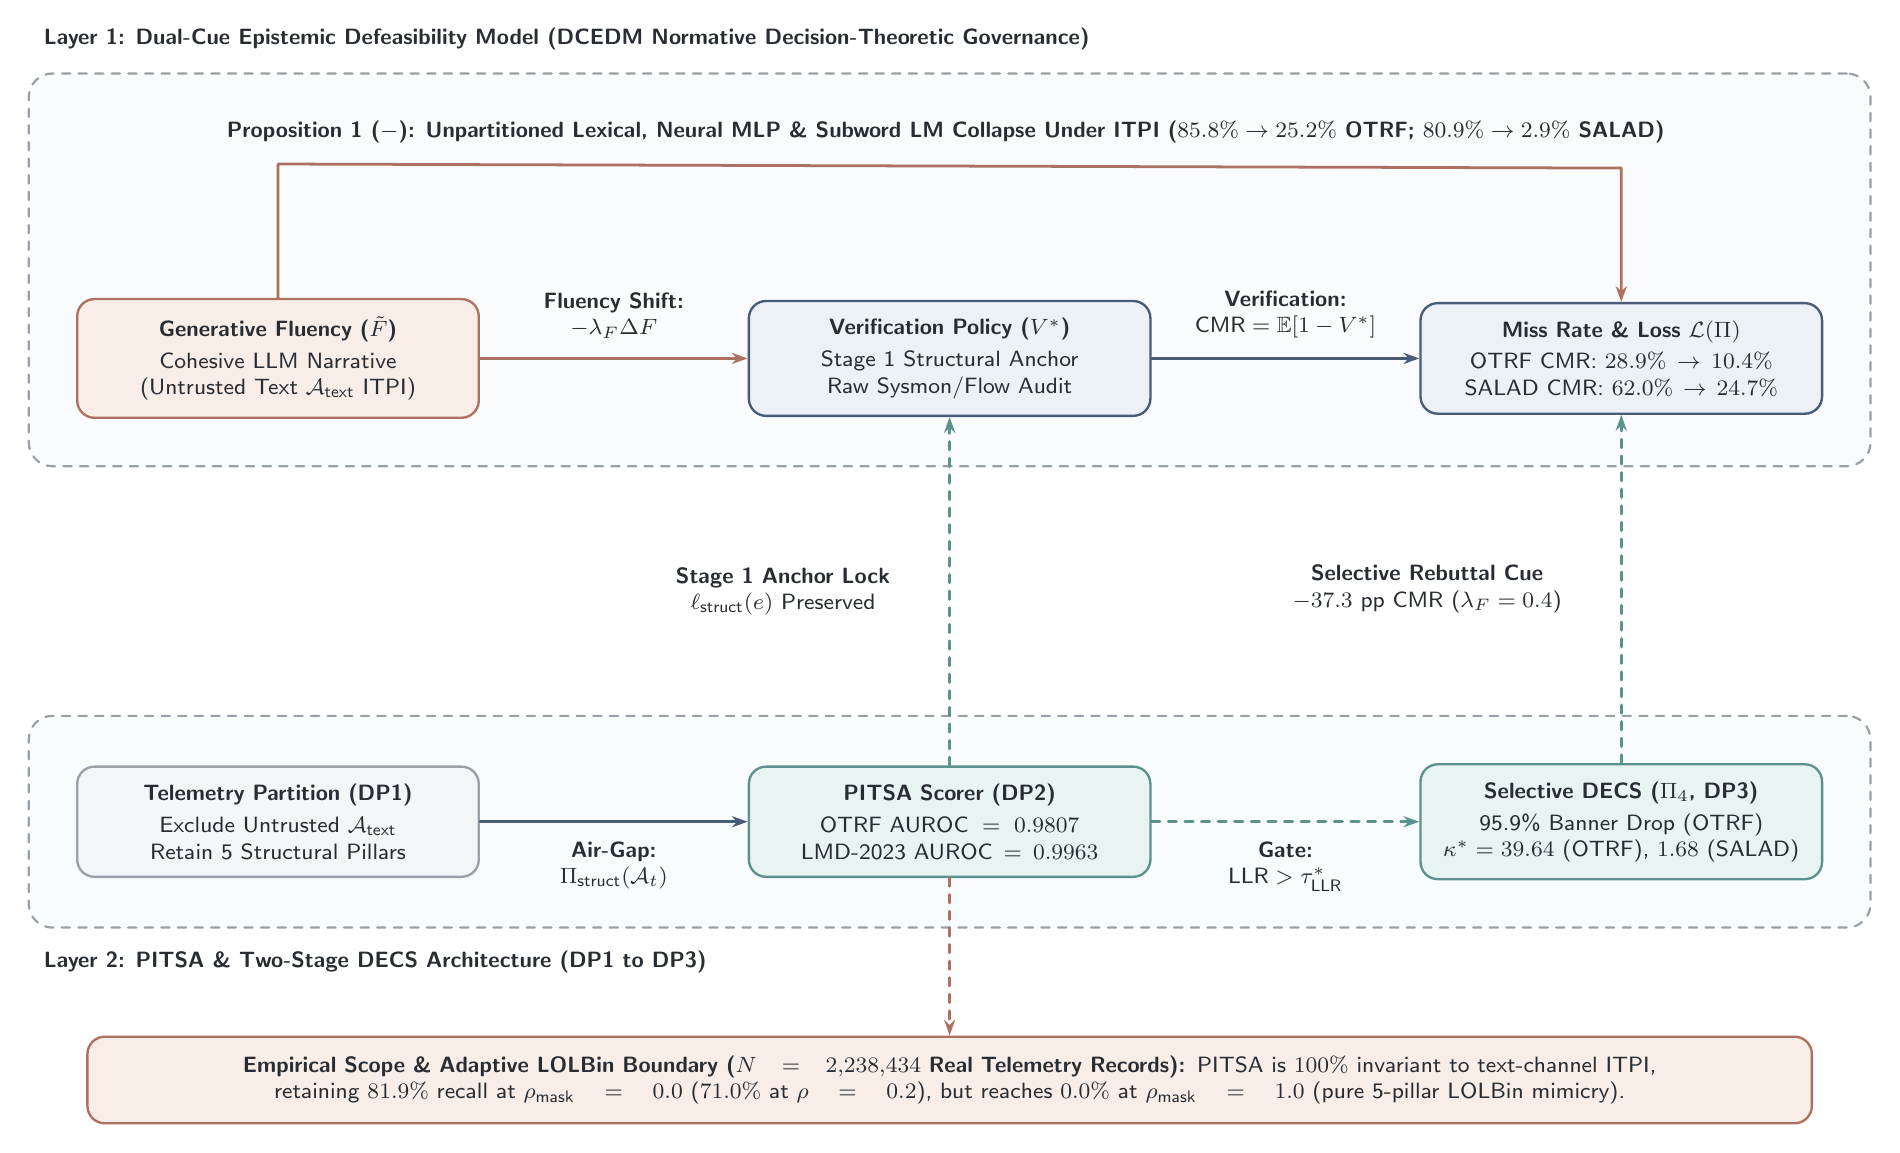
\begin{tikzpicture}[node distance=20mm and 22mm]

  % Top Row: Layer 1 (DCEDM Decision-Theoretic Mechanism)
  \node[caution] (fluency) {
    \textbf{Generative Fluency ($\tilde{F}$)}\\[2pt]
    Cohesive LLM Narrative\\
    (Untrusted Text $\mathcal{A}_{\text{text}}$ ITPI)
  };

  \node[primary, right=34mm of fluency] (vdepth) {
    \textbf{Verification Policy ($V^*$)}\\[2pt]
    Stage 1 Structural Anchor\\
    Raw Sysmon/Flow Audit
  };

  \node[primary, right=34mm of vdepth] (override) {
    \textbf{Miss Rate \& Loss $\mathcal{L}(\Pi)$}\\[2pt]
    OTRF CMR: $28.9\% \rightarrow 10.4\%$\\
    SALAD CMR: $62.0\% \rightarrow 24.7\%$
  };

  % Direct arc high above Layer 1
  \coordinate (h2_left) at ($(fluency.north)+(0,17mm)$);
  \coordinate (h2_right) at ($(override.north)+(0,17mm)$);
  \draw[caution-flow] (fluency.north) to (h2_left) to (h2_right) to (override.north);
  \node[label, anchor=south] (h2_label) at ($(h2_left)!0.5!(h2_right)+(0,2.8mm)$) {
    \textbf{Proposition 1 ($-$): Unpartitioned Lexical, Neural MLP \& Subword LM Collapse Under ITPI ($85.8\% \rightarrow 25.2\%$ OTRF; $80.9\% \rightarrow 2.9\%$ SALAD)}
  };

  % Bottom Row: Layer 2 (PITSA + DECS Socio-Technical Artifact)
  \node[neutral, below=44mm of fluency] (telemetry) {
    \textbf{Telemetry Partition (DP1)}\\[2pt]
    Exclude Untrusted $\mathcal{A}_{\text{text}}$\\
    Retain 5 Structural Pillars
  };

  \node[context, right=34mm of telemetry] (pitsa) {
    \textbf{PITSA Scorer (DP2)}\\[2pt]
    OTRF $\text{AUROC}=0.9807$\\
    LMD-2023 $\text{AUROC}=0.9963$
  };

  \node[context, right=34mm of pitsa] (decs) {
    \textbf{Selective DECS ($\Pi_4$, DP3)}\\[2pt]
    95.9\% Banner Drop (OTRF)\\
    $\kappa^*=39.64$ (OTRF), $1.68$ (SALAD)
  };

  % Boundary / Threat Scope Node below PITSA
  \node[caution, below=20mm of pitsa, text width=214mm, minimum height=11mm] (boundary) {
    \textbf{Empirical Scope \& Adaptive LOLBin Boundary ($N=2{,}238{,}434$ Real Telemetry Records):} PITSA is $100\%$ invariant to text-channel ITPI,\\
    retaining $81.9\%$ recall at $\rho_{\text{mask}}=0.0$ ($71.0\%$ at $\rho=0.2$), but reaches $0.0\%$ at $\rho_{\text{mask}}=1.0$ (pure 5-pillar LOLBin mimicry).
  };

  % Background layer grouping
  \begin{scope}[on background layer]
    \node[group, fill=PaleBlue!25, fit=(fluency) (vdepth) (override) (h2_left) (h2_right) (h2_label)] (dcedm_box) {};
    \node[group, fill=PaleTeal!25, fit=(telemetry) (pitsa) (decs)] (artifact_box) {};
  \end{scope}

  % Layer 1 and Layer 2 titles placed cleanly outside dashed containers without crossing center arrow
  \node[label, anchor=south west] (l1_title) at ($(dcedm_box.north west)+(2mm,2.8mm)$) {
    \textbf{Layer 1: Dual-Cue Epistemic Defeasibility Model (DCEDM Normative Decision-Theoretic Governance)}
  };

  \node[label, anchor=north west] at ($(artifact_box.south west)+(2mm,-2.8mm)$) {
    \textbf{Layer 2: PITSA \& Two-Stage DECS Architecture (DP1 to DP3)}
  };

  % Horizontal Connectors in Layer 1
  \draw[caution-flow] (fluency.east) to (vdepth.west);
  \node[label, anchor=south] at ($(fluency.east)!0.5!(vdepth.west)+(0,2.5mm)$) {
    \textbf{Fluency Shift:}\\$-\lambda_F \Delta F$
  };

  \draw[flow] (vdepth.east) to (override.west);
  \node[label, anchor=south] at ($(vdepth.east)!0.5!(override.west)+(0,2.5mm)$) {
    \textbf{Verification:}\\$\text{CMR} = \mathbb{E}[1-V^*]$
  };

  % Horizontal Connectors in Layer 2
  \draw[flow] (telemetry.east) to (pitsa.west);
  \node[label, anchor=north] at ($(telemetry.east)!0.5!(pitsa.west)+(0,-2.5mm)$) {
    \textbf{Air-Gap:}\\$\Pi_{\text{struct}}(\mathcal{A}_t)$
  };

  \draw[contextual-flow] (pitsa.east) to (decs.west);
  \node[label, anchor=north] at ($(pitsa.east)!0.5!(decs.west)+(0,-2.5mm)$) {
    \textbf{Gate:}\\$\text{LLR} > \tau^*_{\text{LLR}}$
  };

  % Vertical Cross-Layer Connectors
  \draw[contextual-flow] (pitsa.north) to (vdepth.south);
  \node[label, anchor=east] at ($(pitsa.north)!0.50!(vdepth.south)+(-7.5mm,0)$) {
    \textbf{Stage 1 Anchor Lock}\\
    $\ell_{\text{struct}}(e)$ Preserved
  };

  \draw[contextual-flow] (decs.north) to (override.south);
  \node[label, anchor=east] at ($(decs.north)!0.50!(override.south)+(-7.5mm,0)$) {
    \textbf{Selective Rebuttal Cue}\\
    $-37.3\text{ pp}$ CMR ($\lambda_F=0.4$)
  };

  % Boundary link
  \draw[caution-flow, dashed] (pitsa.south) to (boundary.north);

\end{tikzpicture}
\end{document}
